\documentclass[12pt,a4paper]{article}
\usepackage[a4paper,margin=1in]{geometry}
\usepackage{graphicx}
\usepackage{booktabs}
\usepackage{amsmath,amssymb}
\usepackage{float}
\usepackage{hyperref}
\usepackage{xcolor}
\usepackage{listings}
\usepackage{enumitem}
\usepackage{fancyhdr}
\usepackage{longtable}
\hypersetup{colorlinks=true,linkcolor=blue,urlcolor=blue}
\pagestyle{fancy}
\fancyhf{}
\lhead{ICS1512}
\rhead{Machine Learning Algorithms Laboratory}
\cfoot{\thepage}
\lstset{
language=Python,
basicstyle=\ttfamily\small,
numbers=left,
frame=single,
breaklines=true,
showstringspaces=false
}
\begin{document}
\begin{tabular}{|p{4cm}|p{11cm}|}
\hline
Experiment No. & 4 \\ \hline
Experiment Title & Binary Classification using Linear and Kernel-Based Models
\footnote{\textbf{GitHub Repository: }\url{https://github.com/username/repository}}\\ \hline
Student Name & T.Ashwath Ram\\ \hline
Register Number & 3122247001007\\ \hline
Faculty & Dr. Poreddy Ajay Kumar Reddy \\ \hline
Submission Date & 25.07.2026 \\ \hline
\end{tabular}

\section{Objective}
To classify emails as spam or ham using Logistic Regression and Support Vector Machine (SVM)
classifiers, and to analyze the effect of hyperparameter tuning (regularization strength,
solver, kernel choice) on classification performance, comparing a linear probabilistic model
against a margin-based kernel model.

\section{Problem Statement}
Given a 57-dimensional numeric feature vector describing an email (word frequencies, character
frequencies, and capital-letter run-length statistics), the task is to predict a binary label:
\textbf{spam (1)} or \textbf{ham (0)}. Two classification paradigms are compared: Logistic
Regression, a linear probabilistic classifier, and SVM, a margin-based classifier evaluated
across four kernels (Linear, Polynomial, RBF, Sigmoid).

\section{Theory}

\subsection*{Logistic Regression}
Logistic Regression models the probability that a sample belongs to the positive class using the
sigmoid function:
\begin{equation}
P(y=1 \mid x) = \frac{1}{1 + e^{-(w^T x + b)}}
\end{equation}
A threshold (0.5 by default) converts this probability into a class label. The model is trained
by minimizing log-loss (cross-entropy loss). Regularization controls overfitting: \textbf{L1
(Lasso)} shrinks some coefficients exactly to zero, performing implicit feature selection;
\textbf{L2 (Ridge)} shrinks all weights but keeps every feature. The inverse regularization
strength $C$ trades off model complexity against regularization -- small $C$ gives strong
regularization and a simpler model, large $C$ gives weak regularization and a more complex model.
The \texttt{liblinear} solver suits small datasets and supports both L1 and L2, while
\texttt{saga} is efficient on large datasets and also supports both penalties.

\subsection*{Support Vector Machine (SVM)}
SVM finds the hyperplane that maximizes the margin between the two classes; only the points
closest to the boundary (support vectors) determine it. Four kernels were compared:
\textbf{Linear} (suitable for linearly separable data), \textbf{Polynomial} (captures polynomial
feature interactions), \textbf{RBF} (handles complex non-linear boundaries), and \textbf{Sigmoid}
(functionally similar to a neural network activation). Its hyperparameters are $C$ (small $C$
gives a wider margin and higher bias; large $C$ gives a narrower margin and lower bias) and
$\gamma$ (controls the influence radius of a single training point for the RBF/polynomial/sigmoid
kernels).

\subsection*{Hyperparameter Tuning}
\textbf{Grid Search} exhaustively evaluates every combination of predefined hyperparameters under
cross-validation; \textbf{Randomized Search} samples a random subset of combinations and is more
computationally efficient on large search spaces. This experiment used Grid Search (via
\texttt{GridSearchCV}) for both models.

\section{Dataset Description}
\begin{longtable}{|p{6cm}|p{8cm}|}
\hline
Dataset Name & Spambase \\ \hline
Dataset Source & Kaggle -- \url{https://www.kaggle.com/datasets/somesh24/spambase} \\ \hline
Number of Samples & 4{,}601 (raw); 4{,}210 after removing 391 duplicate rows \\ \hline
Number of Features & 57 numeric features (48 word-frequency, 6 character-frequency, 3
capital-run-length statistics) \\ \hline
Number of Classes & 2 (Spam = 1, Ham = 0) -- class distribution after deduplication: 2{,}531 Ham
(60.12\%), 1{,}679 Spam (39.88\%) \\ \hline
Missing Values & None (0 missing values confirmed across all 58 columns) \\ \hline
Train-Test Split & 80\% / 20\%, stratified on class (3{,}368 training samples / 842 test samples),
random\_state = 42 \\ \hline
\end{longtable}

\section{Exploratory Data Analysis}

\begin{figure}[H]
\centering
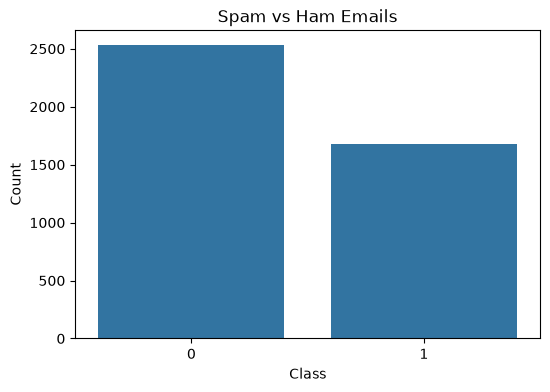
\includegraphics[width=0.55\linewidth]{figures/fig_class_dist.png}
\caption{Class distribution -- Spam vs. Ham}
\end{figure}
\textbf{Inference:} The dataset shows a moderate class imbalance, with ham emails (60.1\%)
outnumbering spam (39.9\%). This imbalance is mild enough that accuracy remains informative, but
precision and recall are tracked separately per class to confirm the models are not simply biased
toward predicting the majority (ham) class.

\begin{figure}[H]
\centering
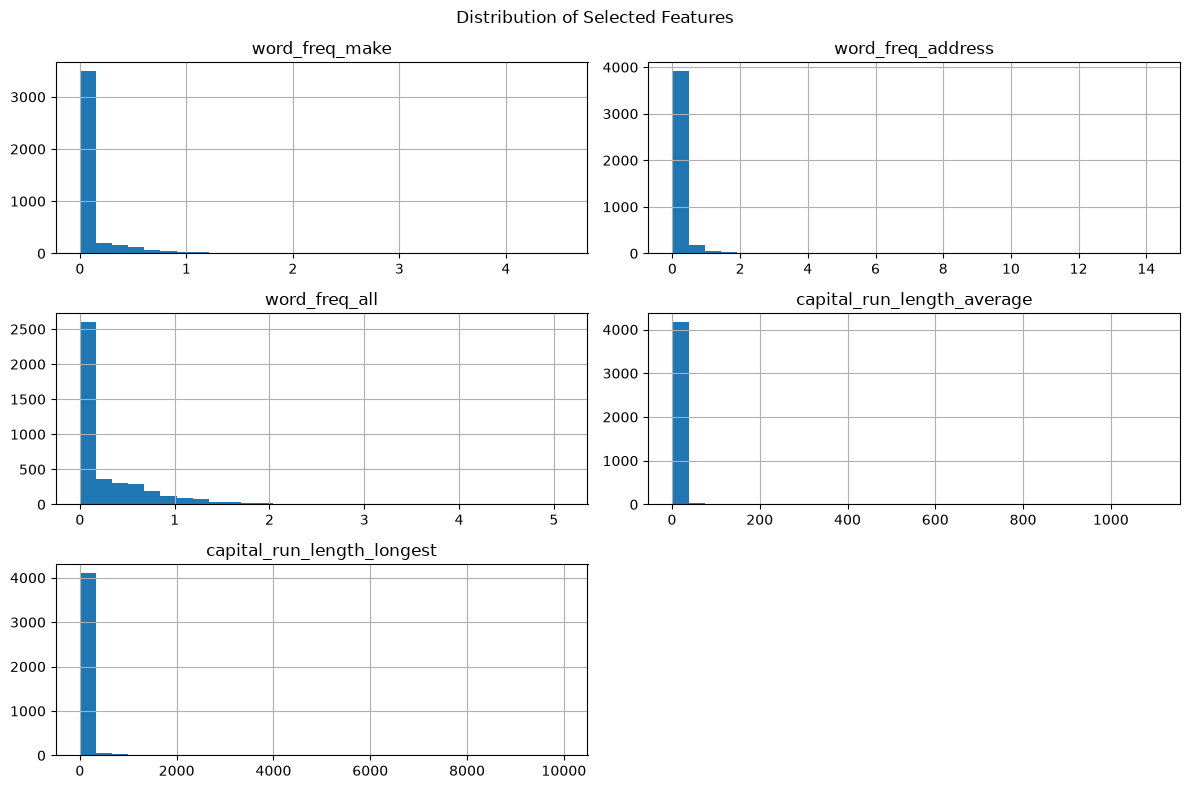
\includegraphics[width=0.85\linewidth]{figures/fig_hist_features.png}
\caption{Distribution of selected features (word\_freq\_make, word\_freq\_address,
word\_freq\_all, capital\_run\_length\_average, capital\_run\_length\_longest)}
\end{figure}
\textbf{Inference:} All five features are heavily right-skewed, with most emails scoring near
zero and a long tail of high values. This is typical of word-frequency and capitalization
features in spam datasets, and motivates feature scaling before training distance/margin-based
models such as SVM.

\begin{figure}[H]
\centering
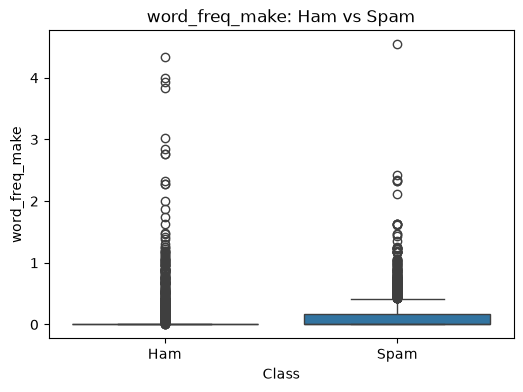
\includegraphics[width=0.6\linewidth]{figures/fig_box_make.png}
\caption{Boxplot of word\_freq\_make by class (Ham vs. Spam)}
\end{figure}
\textbf{Inference:} Spam emails show a slightly higher median and more high-value outliers for
``make'' than ham emails, though the separation is not dramatic on its own. This is consistent
with the pattern across most individual word-frequency features -- weak-to-moderate discriminative
power that becomes strong only when combined across all 57 features.

\begin{figure}[H]
\centering
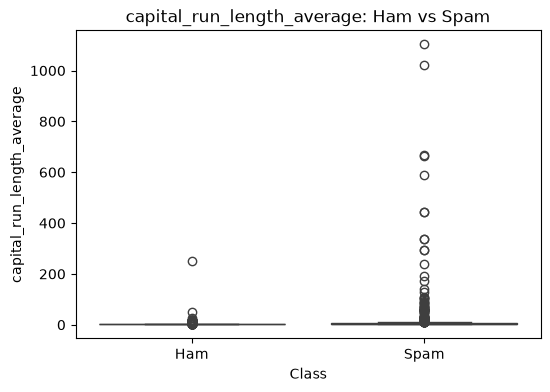
\includegraphics[width=0.6\linewidth]{figures/fig_box_caprun.png}
\caption{Boxplot of capital\_run\_length\_average by class (Ham vs. Spam)}
\end{figure}
\textbf{Inference:} Spam emails show a visibly wider spread and higher outlier values in average
capital-run length than ham emails, consistent with spam's tendency to use capitalized text for
emphasis. This feature appears to be one of the more individually discriminative predictors in the
dataset.

\begin{figure}[H]
\centering
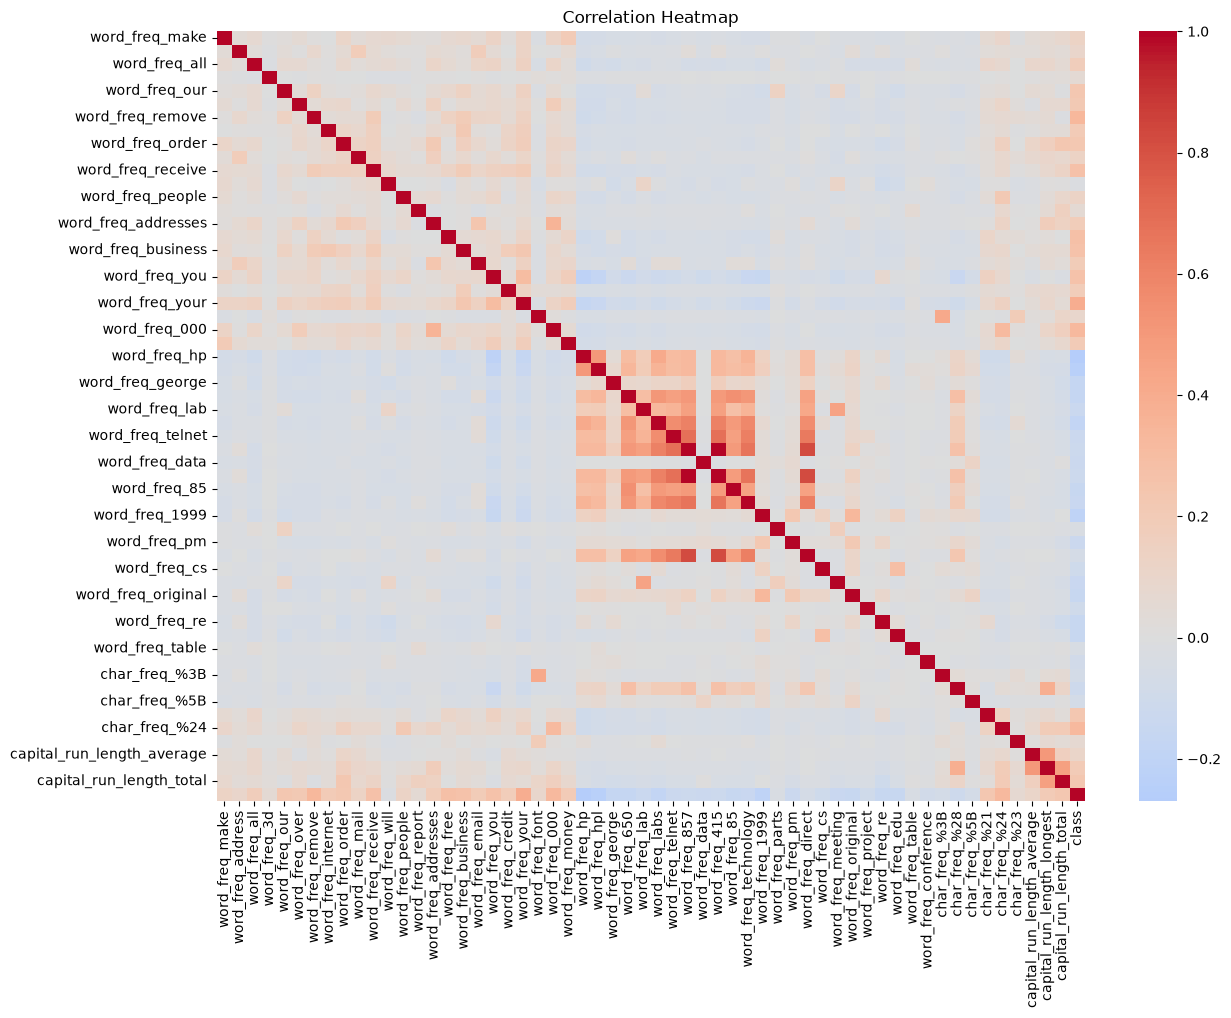
\includegraphics[width=0.85\linewidth]{figures/fig_corr_heatmap.png}
\caption{Correlation heatmap of all numeric features}
\end{figure}
\textbf{Inference:} A cluster of technical/business-related word frequencies
(\texttt{word\_freq\_hp}, \texttt{hpl}, \texttt{650}, \texttt{lab}, \texttt{labs}, \texttt{telnet},
\texttt{857}, \texttt{415}, \texttt{85}, \texttt{technology}, \texttt{direct}) shows moderate
mutual correlation, while most remaining features are weakly correlated with each other. Low
overall multicollinearity is favorable for both Logistic Regression's coefficient stability and
SVM's margin computation.

\section{Data Preprocessing}
\begin{itemize}
\item \textbf{Missing value handling:} Verified with \texttt{df.isnull().sum()}; zero missing
values were found across all 58 columns, so no imputation was required.
\item \textbf{Duplicate removal:} 391 duplicate rows were identified and dropped
(\texttt{drop\_duplicates}), reducing the dataset from 4{,}601 to 4{,}210 rows.
\item \textbf{Feature/target separation:} The \texttt{class} column was separated as target $y$;
the remaining 57 columns formed feature matrix $X$.
\item \textbf{Train-test split:} An 80/20 stratified split (\texttt{stratify=y},
\texttt{random\_state=42}) was used, yielding 3{,}368 training and 842 test samples, preserving
the class ratio in both splits.
\item \textbf{Feature scaling:} \texttt{StandardScaler} was fit on the training split and applied
to both training and test splits before training either Logistic Regression or SVM.
\end{itemize}

\section{Experimental Setup}
\begin{tabular}{ll}
\toprule
Python Version & 3.13.15 \\
Scikit-Learn Version & 1.8.0 \\
IDE & Jupyter Notebook \\
Operating System & Windows \\
Hardware & Personal laptop (CPU-only) \\
\bottomrule
\end{tabular}

\section{Hyperparameter Selection}
\begin{tabular}{ll}
\toprule
Parameter & Value\\
\midrule
LR search space -- Regularization & L1, L2 \\
LR search space -- $C$ & $\{0.01, 0.1, 1, 10, 100\}$ \\
LR search space -- Solver & liblinear, saga \\
SVM search space -- Kernel & Linear, Polynomial, RBF, Sigmoid \\
SVM search space -- $C$ & $\{0.1, 1, 10, 100\}$ \\
SVM search space -- $\gamma$ & scale, auto \\
SVM search space -- Degree (Polynomial) & $\{2, 3, 4\}$ \\
\bottomrule
\end{tabular}

\section{Results}

\subsection*{Hyperparameter Tuning Results}
\begin{longtable}{p{3cm}p{3cm}p{5cm}p{2.5cm}}
\toprule
Model & Search Method & Best Parameters & Best CV Accuracy \\
\midrule
Logistic Regression & Grid Search & $C=1$, penalty = L1, solver = liblinear & 0.9243 \\
SVM & Grid Search & $C=10$, $\gamma$ = scale, kernel = RBF & 0.9255 \\
\bottomrule
\end{longtable}
\textit{Note: only Grid Search was used for both models in this experiment (Randomized Search was
not run), per the lab manual's allowance to use either method.}

\subsection*{Logistic Regression Performance}
\begin{tabular}{lcc}
\toprule
Metric & Baseline (default) & Tuned (Grid Search) \\
\midrule
Accuracy & 0.9347 & 0.9371 \\
Precision & 0.9297 & 0.9301 \\
Recall & 0.9048 & 0.9107 \\
F1 Score & 0.9170 & 0.9203 \\
Training Time (s) & Not explicitly timed & Not explicitly timed \\
\bottomrule
\end{tabular}

\subsection*{SVM Kernel-wise Performance (default $C=1$, $\gamma$=scale)}
\begin{longtable}{lccc}
\toprule
Kernel & Accuracy & F1 Score & Training Time (s) \\
\midrule
Linear & 0.9359 & 0.9189 & 0.6736 \\
Polynomial & 0.7660 & 0.5988 & 0.6735 \\
RBF & 0.9323 & 0.9135 & 0.3657 \\
Sigmoid & 0.8967 & 0.8676 & 0.3398 \\
\bottomrule
\end{longtable}

\begin{tabular}{lc}
\toprule
Tuned SVM (best: RBF, $C=10$, $\gamma$=scale) & Value \\
\midrule
Accuracy & 0.9335 \\
Precision & 0.9294 \\
Recall & 0.9018 \\
F1 Score & 0.9154 \\
\bottomrule
\end{tabular}

\subsection*{K-Fold Cross-Validation Results (K = 5, StratifiedKFold, tuned models)}
\begin{longtable}{lcc}
\toprule
Fold & Logistic Regression & SVM \\
\midrule
Fold 1 & 0.9276 & 0.9276 \\
Fold 2 & 0.9418 & 0.9382 \\
Fold 3 & 0.9264 & 0.9311 \\
Fold 4 & 0.9145 & 0.9169 \\
Fold 5 & 0.9181 & 0.9252 \\
\midrule
Average & 0.9257 & 0.9278 \\
\bottomrule
\end{longtable}

\section{Result Visualization}

\begin{figure}[H]
\centering
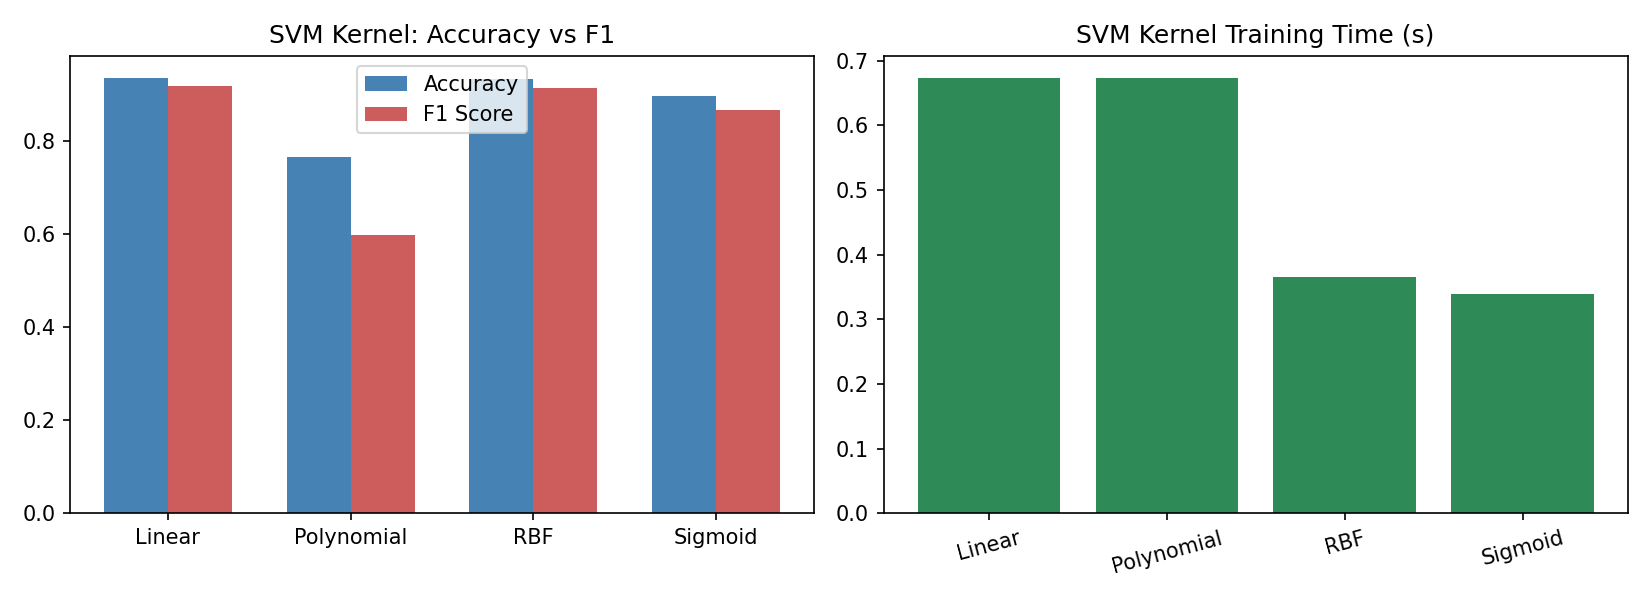
\includegraphics[width=0.9\linewidth]{figures/fig_svm_kernel_comparison.png}
\caption{SVM kernel comparison: Accuracy/F1 (left) and training time (right)}
\end{figure}
\textbf{Inference:} The Polynomial kernel is a clear outlier, with both accuracy (0.766) and F1
(0.599) far below the other three kernels, indicating it is a poor fit for this feature space
under default hyperparameters. Linear and RBF kernels perform almost identically
(accuracy $\approx$ 0.93--0.94), while RBF and Sigmoid train roughly $2\times$ faster than Linear
and Polynomial on this dataset.

\begin{figure}[H]
\centering
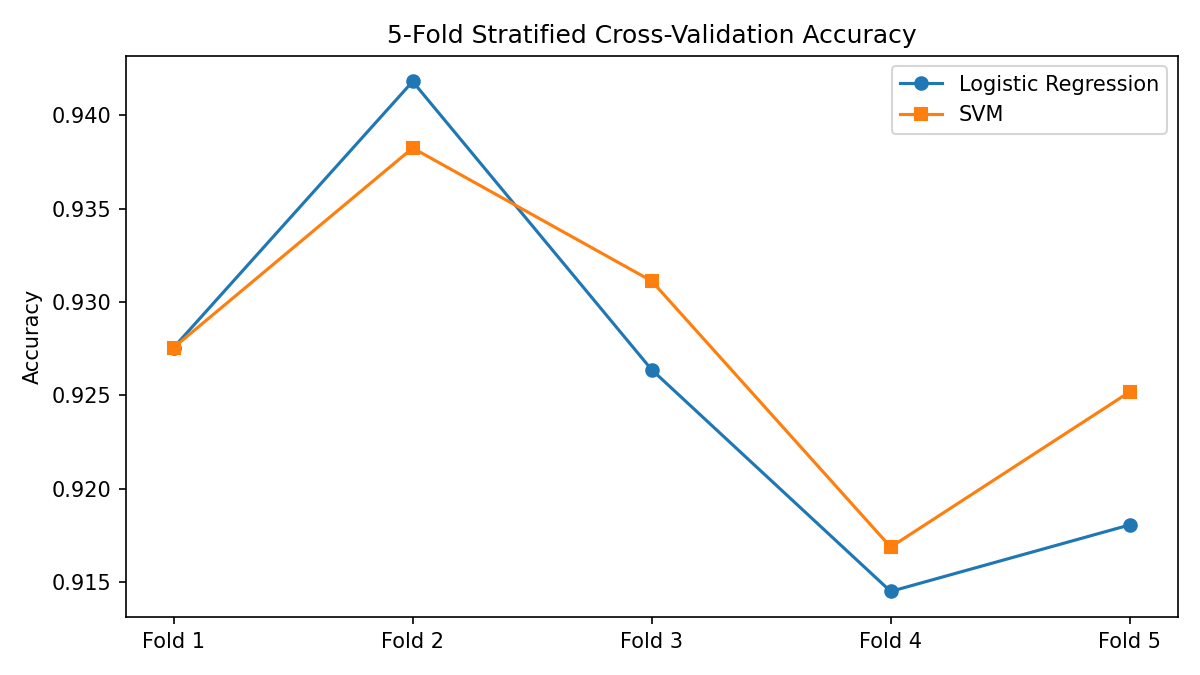
\includegraphics[width=0.7\linewidth]{figures/fig_cv_folds.png}
\caption{5-fold stratified cross-validation accuracy: Logistic Regression vs. SVM}
\end{figure}
\textbf{Inference:} The two models track each other closely across folds, with SVM ahead in three
of five folds and tied in one. Fold 4 is the weakest for both models (0.9145 and 0.9169
respectively), suggesting that fold contains a subset of emails that are inherently harder to
classify for both linear and kernel-based approaches alike -- i.e., the difficulty is shared
across model types rather than being model-specific.

\begin{figure}[H]
\centering
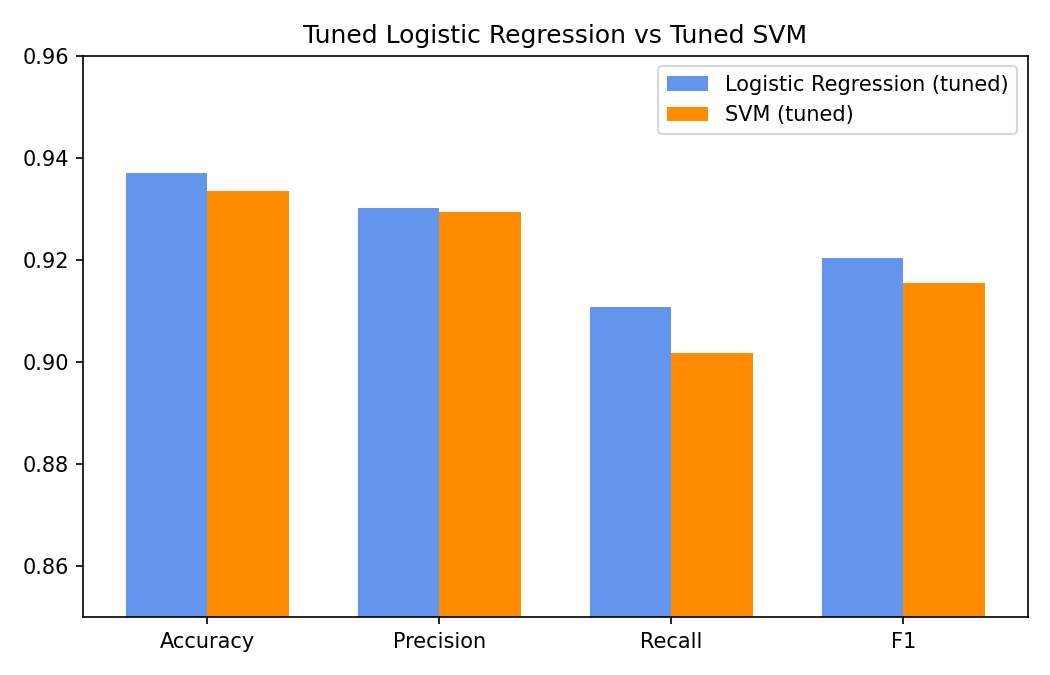
\includegraphics[width=0.75\linewidth]{figures/fig_lr_vs_svm.png}
\caption{Tuned Logistic Regression vs. tuned SVM -- test set metrics}
\end{figure}
\textbf{Inference:} Tuned Logistic Regression edges out tuned SVM on every test-set metric
(accuracy, precision, recall, and F1), though the margins are small (0.4--0.9 percentage points).
Combined with the cross-validation result where SVM was marginally ahead on average, this suggests
the two models are practically comparable on this dataset, with the single train-test split
slightly favoring Logistic Regression by chance.

\section{Comparative Analysis}

\subsection*{Observations}
\begin{itemize}
\item \textbf{Best-performing classifier:} On the held-out test split, tuned Logistic Regression
is marginally best (Accuracy 0.9371 vs. SVM's 0.9335); on 5-fold cross-validation, tuned SVM is
marginally best on average (0.9278 vs. 0.9257). The two models are effectively tied within normal
fold-to-fold variance, with Logistic Regression having a slight edge in precision/recall balance
and simplicity.
\item \textbf{Impact of regularization:} Grid Search selected L1 regularization at a moderate
$C=1$ for Logistic Regression, improving test accuracy from 0.9347 (baseline, unregularized
default) to 0.9371 and CV accuracy to 0.9243 -- a modest but consistent gain, with L1's implicit
feature selection likely helping given the large number of weak individual word-frequency
predictors observed in the EDA.
\item \textbf{Kernel behavior in SVM:} RBF was selected as the best kernel after tuning (CV
accuracy 0.9255), consistent with its strong default-hyperparameter performance (0.9323 accuracy).
The Polynomial kernel's poor default performance (0.766 accuracy) shows that not all kernels are
equally suited to this feature space without careful degree/gamma tuning; increasing $C$ to 10
for the tuned RBF model narrowed the margin, trading some bias for reduced misclassification on
the training data.
\item \textbf{Bias--variance trade-off:} Logistic Regression, as a linear model, has higher bias
but lower variance -- it generalizes consistently across folds (0.9145--0.9418 range across CV
folds) without needing extensive tuning. SVM with an RBF kernel has lower bias (able to fit more
complex boundaries) but showed comparable fold-to-fold variance (0.9169--0.9382) here, indicating
that with proper regularization ($C=10$, not too large), it avoided the higher variance that
kernel methods can otherwise be prone to.
\end{itemize}

\begin{table}[H]
\centering
\begin{tabular}{lcc}
\toprule
Criterion & Logistic Regression & SVM \\
\midrule
Accuracy & 0.9371 (test) / 0.9257 (CV avg) & 0.9335 (test) / 0.9278 (CV avg) \\
Model Complexity & Low & High \\
Training Time & Low & High \\
Interpretability & High & Low \\
\bottomrule
\end{tabular}
\caption{Comparative summary of Logistic Regression and SVM}
\end{table}

\section{Learning Outcomes}
\begin{itemize}
\item Understood the mechanics of probabilistic (Logistic Regression) and margin-based (SVM)
binary classifiers, including their respective decision-boundary formulations.
\item Applied Grid Search hyperparameter tuning to both models, observing measurable (if modest)
accuracy improvements over untuned baselines.
\item Evaluated classification models using accuracy, precision, recall, and F1 score, and
cross-validated results using 5-fold stratified cross-validation for a more reliable performance
estimate than a single train-test split.
\item Interpreted experimental results in light of theory -- e.g., connecting the Polynomial
kernel's poor default performance to its sensitivity to hyperparameters, and Logistic Regression's
L1 regularization to the presence of many weakly-informative features in the dataset.
\end{itemize}

\section{Conclusion}
Both Logistic Regression and SVM achieve strong, closely-matched performance on the Spambase
spam-classification task (test accuracy 0.934--0.937, CV accuracy 0.926--0.928). Grid Search
identified L1-regularized Logistic Regression ($C=1$, liblinear) and RBF-kernel SVM ($C=10$,
$\gamma$=scale) as the best configurations for each model family, each improving modestly on
their respective untuned baselines. Given the near-identical accuracy, Logistic Regression is the
more practical choice for this task: it is faster to train, easier to interpret (coefficients
directly indicate each word/character frequency's contribution to the spam decision), and simpler
to deploy and maintain, while SVM's added complexity (kernel choice, $\gamma$ tuning) does not
translate into a meaningful accuracy advantage on this dataset.

\section{References}
\begin{enumerate}
\item Scikit-learn Developers, ``Logistic Regression,'' scikit-learn documentation. [Online].
Available: \url{https://scikit-learn.org/stable/modules/linear_model.html#logistic-regression}
\item Scikit-learn Developers, ``Support Vector Machines,'' scikit-learn documentation. [Online].
Available: \url{https://scikit-learn.org/stable/modules/svm.html}
\item Scikit-learn Developers, ``Tuning the hyper-parameters of an estimator,'' scikit-learn
documentation. [Online]. Available:
\url{https://scikit-learn.org/stable/modules/grid_search.html}
\item Kaggle, ``Spambase Dataset.'' [Online]. Available:
\url{https://www.kaggle.com/datasets/somesh24/spambase}
\item UCI Machine Learning Repository, ``Spambase Data Set.'' [Online]. Available:
\url{https://archive.ics.uci.edu/dataset/94/spambase}
\end{enumerate}

\end{document}
